\documentclass[a4paper]{article}
\usepackage[cm]{fullpage}
\usepackage{url}
\usepackage{listings}
\usepackage{upgreek}
\usepackage{siunitx}
\usepackage{bm}
\usepackage{amsmath}
\usepackage{amsfonts}
\usepackage{graphicx}

\newcommand{\K}{{\mathbb{K}}}
\newcommand{\G}{{\mathbb{G}}}


\usepackage[maxnames=6]{biblatex}
\addbibresource{bibliography.bib}



\title{{\Large \bf GRU} \\ (Geodynamical Rheology Upscaling)}
\author{C. Thieulot \& F. Gueydan}

\begin{document}
\maketitle


%%%%%%%%%%%%%%%%%%%%%%%%%%%%%%%%%%%%%%%%%%%%%%%%%%
\section{Mass and momentum conservation equations}

we start from the mass and momentum conservation equations.
Since our domain is very small gravitational forces are neglected.

\begin{eqnarray}
\vec\nabla \cdot \bm \sigma + \rho \vec{g} &=& \vec{0} \\
\vec\nabla \cdot \vec\upnu &=& 0
\end{eqnarray}

The full stress tensor is given by
\[
\bm\sigma = -p {\bm 1} +  \bm \tau
\]
where ${\bm 1}$ is the unit matrix, $p$ is the pressure and 
${\bm\tau}$ is the deviatoric stress tensor which can be 
written as
\[
\bm\tau = 2 \eta \dot{\bm \varepsilon}(\vec\upnu)
\]
where $\eta$ is the viscosity, $\vec{\upnu}=(u,v)$ is the velocity vector, 
and $\dot{\bm \varepsilon}(\vec\upnu)$ is the (deviatoric) 
strain rate tensor (we assume incompressible flow).

Putting it all together we obtain:
\begin{eqnarray}
-\vec\nabla p + \vec\nabla \cdot (2 \eta \dot{\bm \varepsilon}(\vec\upnu)) + \rho \vec{g} &=& \vec{0} \\
\vec\nabla \cdot \vec\upnu &=& 0
\end{eqnarray}

In what follows we assume the buoyancy forces are negligible, i.e. 
the term $\rho \vec{g}$ is neglected.

For the time being we assume the system is isothermal 
so the energy equation is not solved.


%%%%%%%%%%%%%%%%%%%%%%%%%%%%%%%%%%%%%%%%%%%%%%%%%%
\section{Numerical methods}

The mass and momentum conservation equations are 
solved by means of the FE method. 
$Q_2\times Q_1$ elements are used \cite{thba22}.
The domain is a rectangle of size $L_x \times L_y$
with the lower left corner at $(x,y)=(0,0)$.
The mesh is composed of \lstinline{nelx}$\times$\lstinline{nely} elements.
Boundary conditions are as follows: $\upnu_y=0$ is prescribed on 
all boundaries, while $\upnu_x=\pm \upnu_0$ is prescribed at the 
top and at the bottom (of opposite sign) so that the background 
strain rate is given by 
\[
\dot\varepsilon_b = \frac{\upnu_0}{L_y}
\]
Typically we set $L_y=1~\si{\cm}$ and 
$\dot\varepsilon_b =10^{-15}~\si{\per\second} $ so that 
$\upnu_0= \dot\varepsilon_b L_y \simeq 3.2\cdot 10^{-8}~\si{\cm\per year}$.
Calculations are performed until a strain value $\gamma=2$ 
has been reached, i.e. 
$t_{final} = \gamma/ \dot\varepsilon_b \simeq 2 \times 10^{15}~\si{\second} 
\simeq 64~\si{Myr}$.


\begin{center}
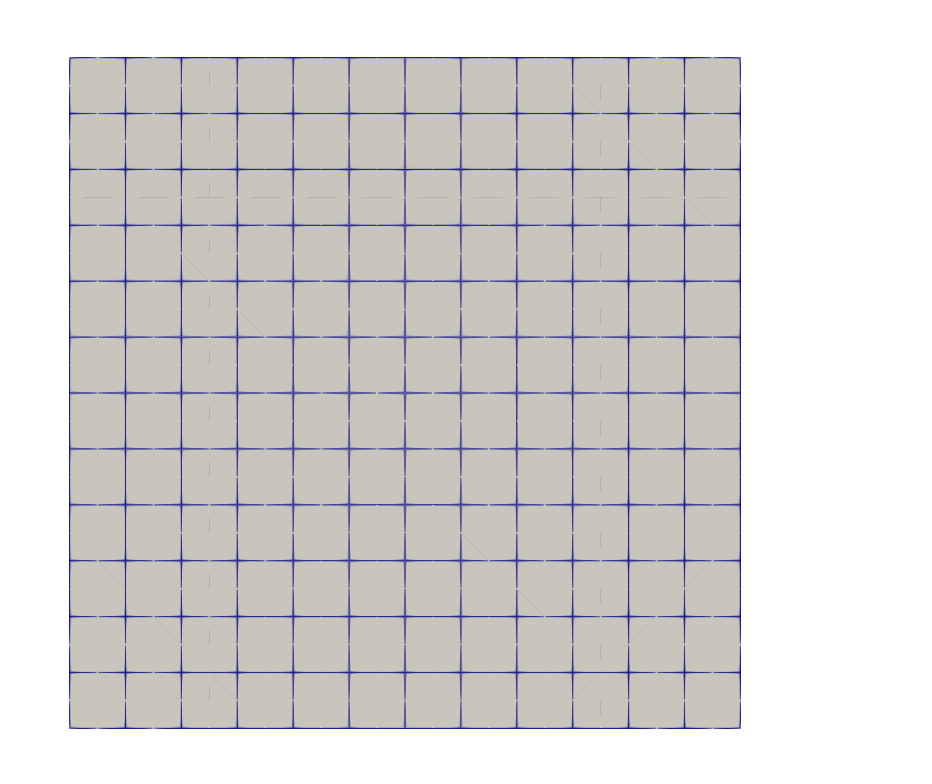
\includegraphics[width=6cm]{images/mesh}
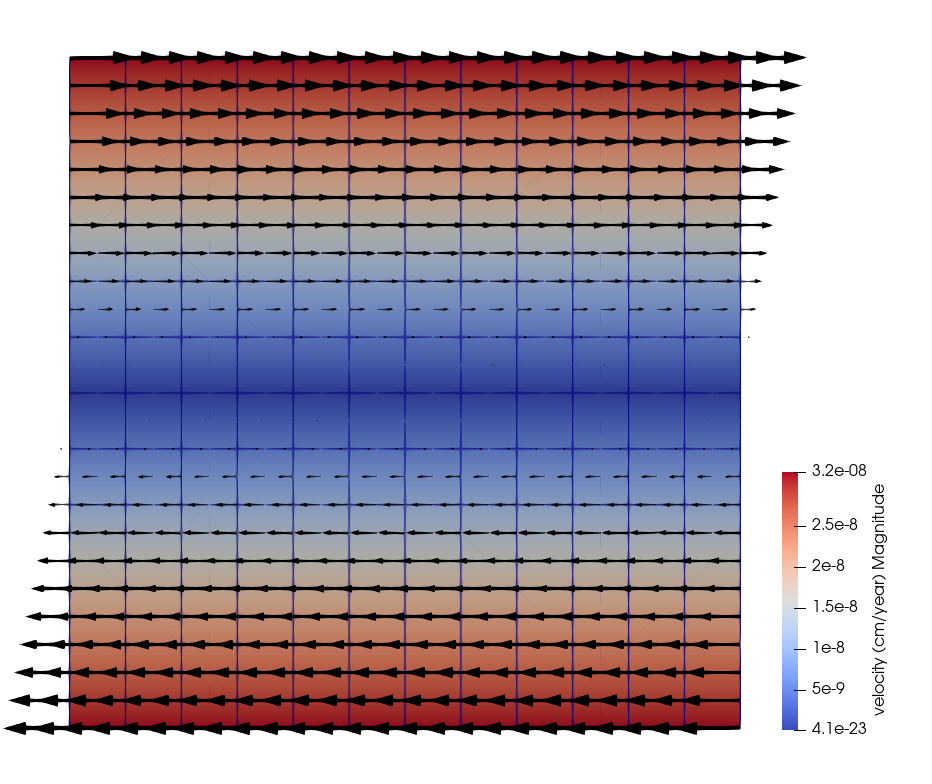
\includegraphics[width=6cm]{images/vel}\\
Left: mesh composed of 12x12 elements. Right: velocity field.
\end{center}

A cloud of passive markers (hereafter called swarm\footnote{\url{https://en.wikipedia.org/wiki/Swarm_behaviour}}) is 
place in the domain. 
The \lstinline{nmarker_per_dim} parameter controls the number of
markers placed in each element at the beginning of the simulation:
\lstinline{nmarker_per_element=nmarker_per_dim**2}
while the total number of markers in the domain is then 
\lstinline{nmarker=nel*nmarker_per_element}.
Markers are initially placed on a regular grid of positions inside each element, as shown 
here: 

\begin{center}
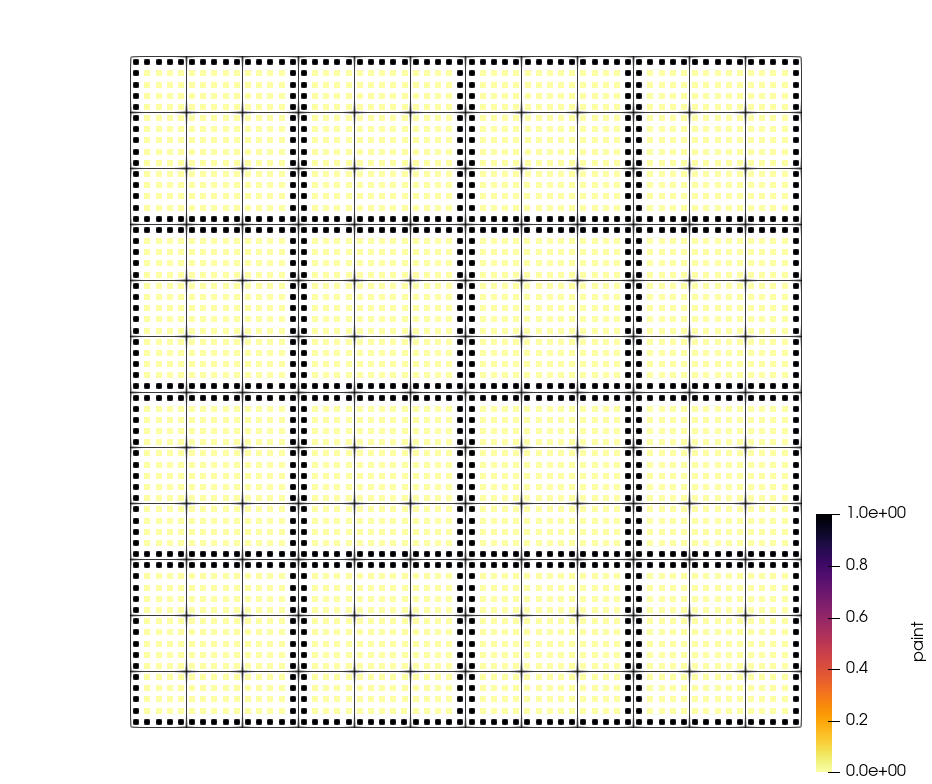
\includegraphics[width=5.6cm]{images/paint}
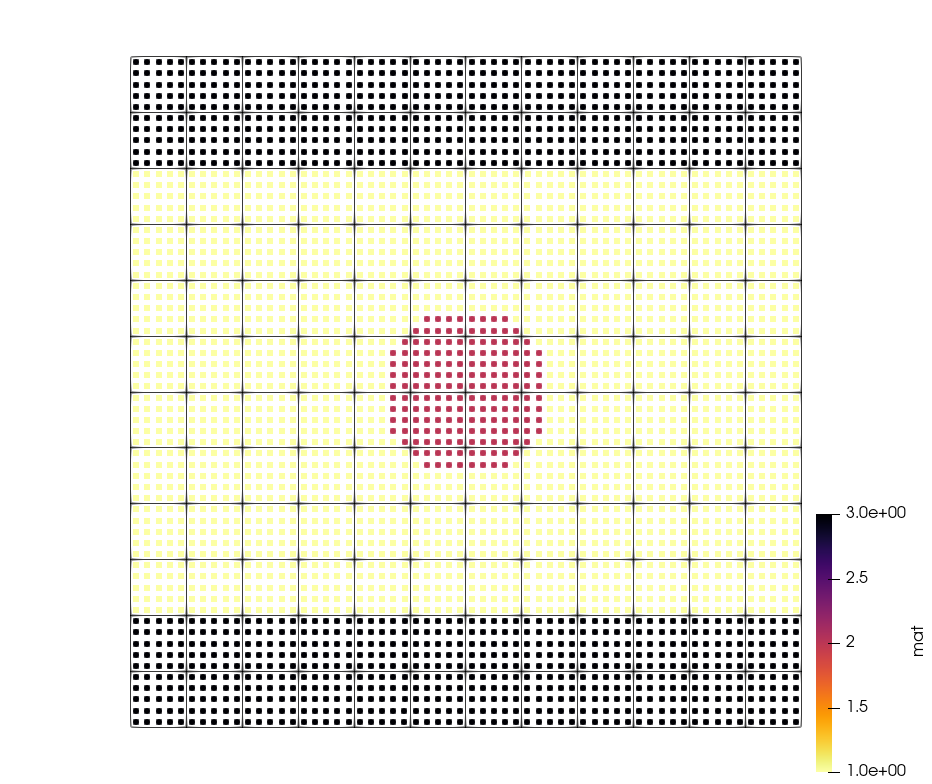
\includegraphics[width=5.6cm]{images/mats}
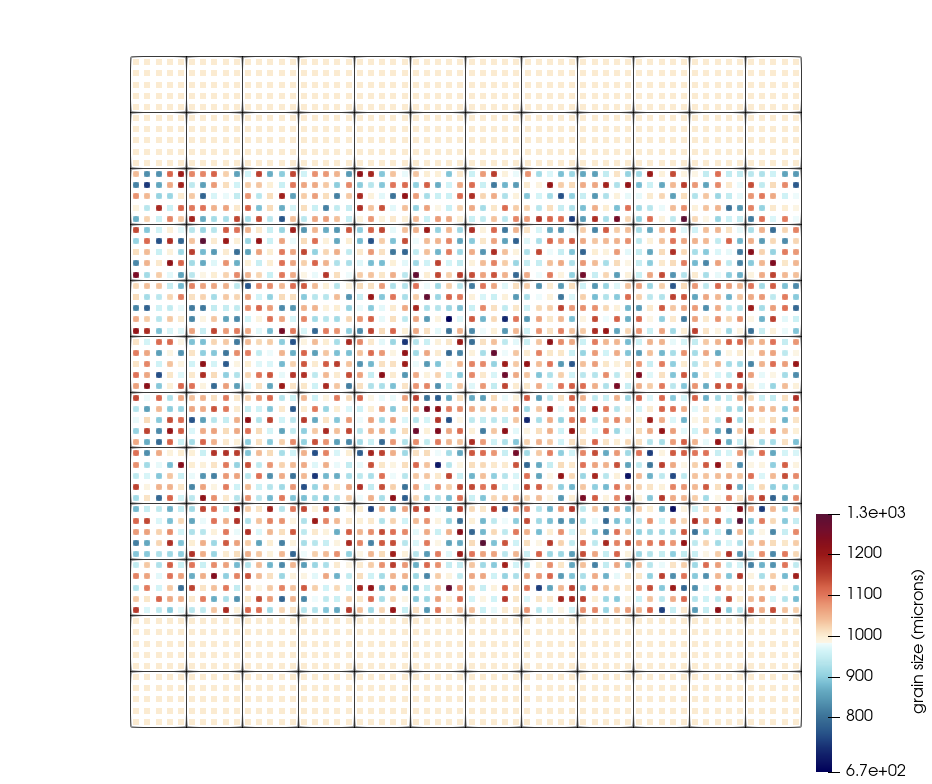
\includegraphics[width=5.6cm]{images/gs}\\
Marker distribution at $t=0$. From left to right: paint, mat, grain size.
Each element contains 5x5 markers.
\end{center}

At the beginning each marker is assigned a grain size $d=1000~\si{\micro\meter}$.
In the middle of the domain random noise is added as shown in the figure above.
It is a gaussian distribution with a prescribed standard deviation of 10\%
of the initial background grain size.
The grain size value carried by each marker is evolved according the 
equation presented in Section~\ref{seq:gsev}.

Each marker carries a lot of information stored in the \lstinline{swarm_xxx}
arrays, where xxx stands for the name of the field, such as x,y,gs,eta,exx,exy,... 

At each time step markers are localised (i.e. we find in which element they reside
in, the (effective) strain rate is interpolated onto them and passed as 
argument to the \lstinline{viscosity} function which, based on the 
temperature $T$ and the grain size $d$ of each marker computes the 
effective viscosity (see Section~\ref{sec:visc}).

This viscosity is then averaged inside the element and is used to build
the elemental matrix $K_\eta$. Note that the averaging can be arithmetic,
geometric or harmonic (default).

The FE matrix is assembled using \lstinline{lil_matrix},
converted to CSR format and then passed to a direct solver alongside the rhs vector.
Node that the code is based on the codes available in the educational Fieldstone project
\footnote{https://cedrict.github.io/}
and is therefore not optimised for performance.


Following a standard approach, the discretised Stokes equations yield
the following linear system
\[
\left(
\begin{array}{cc}
\K & \G \\
\G^T & 0 
\end{array}
\right)
\cdot
\left(
\begin{array}{c}
\vec{\cal V} \\ 
\vec{\cal P}
\end{array}
\right)
=
\left(
\begin{array}{c}
\vec{f} \\ 
\vec{h}
\end{array}
\right)
\]
where $\vec{\cal V}$ is the vector containing all velocity degrees of 
freedom (size { NfemV}={NV}*{ ndofV})
and $\vec{\cal P}$ is the vector containing all pressure degrees of freedom 
(size { NfemP}={ NP}*{ ndofP}).



After the FE matrix has been built, the linear system is solved, and 
we have obtained a new velocity and pressure field.

We then proceed to compute the strain rate components on the nodes.
Since a given node belongs to more than one element the nodal values 
are averages of the corner values of neighbouring elements.
The nodal effective strain rate is then computed as follows:
\[
\dot\varepsilon_e = \sqrt{\frac12 (
\dot\varepsilon_{xx}^2+
\dot\varepsilon_{yy}^2)+
\dot\varepsilon_{xy}^2
)} 
\]

Because the effective viscosity of each marker (and therefore each element)
depends on the strain rate, we carry out simple Picard nonlinear iterations 
which stop when the 2-norm of the relative change of the velocity field between two consecutive 
iterations is less than a set tolerance of $10^{-4}$.


The nodal velocity is used to advect the markers. 
For simplicity we resort to an Euler step, i.e.
\[
\vec{\text x}_i(t+\delta t) = \vec{\text x}_i(t) + \vec\upnu_i \; \delta t
\qquad
i=1,...nmarker 
\]
The timestep $\delta t$ is controled by a CFL condition with $C=0.25$:
\[
\delta t = C \frac{h}{\max |\vec\upnu|_\Omega}
\]
where $h$ is the element size and $C\in[0,1[$.




%%%%%%%%%%%%%%%%%%%%%%%%%%%%%%%%%%%
\section{Strain rate decomposition \label{sec:visc}}

%This stone is based on \textcite{gupr14} (2014). 
The strain rate is to be decomposed into its various contributions 
coming from the different deformation mechanisms, dislocation creep,
diffusion creep, disGBS and low-temperature plasticity:
\[
\dot\varepsilon = \dot\varepsilon_{dsl} + \dot\varepsilon_{dif} + 
\dot\varepsilon_{gbs} + \dot\varepsilon_{exp} 
\]
with
\begin{eqnarray}
\dot{\varepsilon}_{dsl}&=&A_{dsl}\exp\left(-\frac{Q_{dsl}}{RT} \right) \tau^{n_{dsl}}  \\
\dot{\varepsilon}_{dif}&=&A_{dif}\exp\left(-\frac{Q_{dif}}{RT} \right) \tau^{n_{dif}} d^{-m_{dif}} \\
\dot{\varepsilon}_{gbs}&=&A_{gbs}\exp\left(-\frac{Q_{gbs}}{RT} \right) \tau^{n_{gbs}} d^{-m_{gbs}} \\
\dot{\varepsilon}_{exp}&=&A_{exp}\exp\left[-\frac{Q_{exp}}{RT} \left(1 -\frac{\tau}{\tau_p}\right)^{n_{exp}} \right]   
\end{eqnarray}
where $d$ is the grain size, $m$ is the grain size exponent, $\tau_p$ is the Peierls stress defined
for low-temperature plasticity.


There is one major problem with the equations above:
Assuming $\dot\varepsilon$ and temperature $T$ known (as well as all the material parameters $A$, $Q$, $n$, ...),
and that the deformation mechanisms are in series and subjected to the same deviatoric stress $\tau$,
we must find $\tau$ such that
\[
{\cal F}(\tau) = \dot\varepsilon -  \dot\varepsilon_{dsl}(\tau) 
-\dot\varepsilon_{dif}(\tau) -\dot\varepsilon_{gbs}(\tau) - \dot\varepsilon_{exp}(\tau) =0
\]
Unfortunately, this equation is non-linear in $\tau$ so that finding its zero(es) is not
straightforward. A Newton-Raphson\footnote{\url{https://en.wikipedia.org/wiki/Newton's_method}}
algorithm is then used. How to build such an algorithm is presented in Section~2.27.22 of FieldStone
but we will here use an existing python function.
We load \lstinline{scipy.optimize} module and use the \lstinline{newton} function\footnote{\url{
https://docs.scipy.org/doc/scipy/reference/generated/scipy.optimize.newton.html}}
which finds a zero of a real or complex function using the Newton-Raphson (or secant or Halley’s) method.
Once $\tau$ (\lstinline{tau_NR}) has been found, it can then be inserted in the strain rate equations above and
the strain rate partitioning is then complete.

Note that the first 3 equations above can be re-written:
\begin{eqnarray}
\tau &=& \left(\frac{\dot{\varepsilon}_{dsl}}{A_{dsl}} \right)^{1/n_{dsl}} \exp\left(\frac{Q_{dsl}}{n_{dsl}RT} \right) \\ 
\tau &=& \left(\frac{\dot{\varepsilon}_{dif}}{A_{dif}} \right)^{1/n_{dif}} \exp\left(\frac{Q_{dsl}}{n_{dif}RT} \right) d^{m_{dif}/n_{dif}} \\
\tau &=& \left(\frac{\dot{\varepsilon}_{gbs}}{A_{gbs}} \right)^{1/n_{gbs}} \exp\left(\frac{Q_{gbs}}{n_{gbs}RT} \right) d^{m_{gbs}/n_{gbs}} 
\end{eqnarray}



%%%%%%%%%%%%%%%%%%%%%%%%%%%%%%%%%%%
\section{Grain size evolution \label{seq:gsev}}

Following \textcite{prgu09}, we simulate a dynamic grain size reduction
by using the following grain size evolution law \textcite{brcp99}, that relates
the rate of change of grain size $\dot{d}$ to the 
deformation rate $\dot{\varepsilon}$ according to

\[
\dot{d} = -\frac{\dot\varepsilon}{\dot\varepsilon_T} (d-d_\infty)
\]
where $d_\infty$ can be defined in multiple ways:
\begin{itemize}
\item in \textcite{brcp99}, it obeys the following piezometric relationship
\[
d_\infty = B \tau^{-p}
\]
where $d_\infty$ is the recrystallized grain size defined
by the field boundary hypothesis

As of now this option is not implemented.

\item in \textcite{prgu09} it is defined as the boundary between
GBS and diff or disl and diff.
In this paper $d_\infty$ is the recrystallized grain size defined
by the field boundary hypothesis
and is  shown on the following figure:

\begin{center}
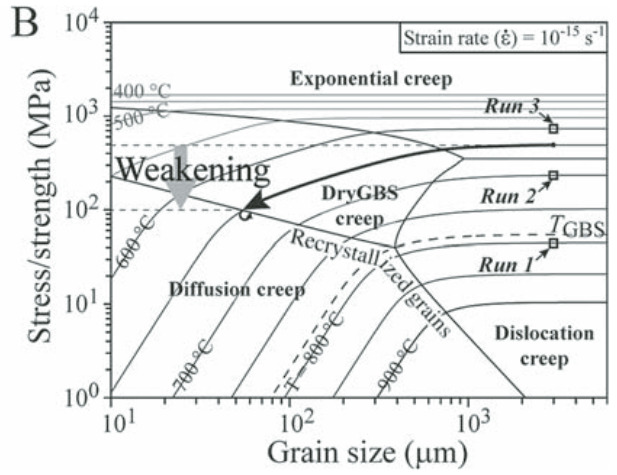
\includegraphics[width=8cm]{images/prgu09}
\end{center}

Let us first consider the GBS-diff boundary. Exactly on the line 
both mechanisms have the same strain rate (50\% of the total strain rate)
and same stress $\tau$ .

\[
\tau
=
\left(\frac{\dot\varepsilon}{A_{dif}}\exp\left(\frac{Q_{dif}}{RT} \right) d^{m_{dif}} \right)^{1/n_{dif}}
=
\left(\frac{\dot\varepsilon}{A_{gbs}} \exp\left(\frac{Q_{gbs}}{RT} \right)  d^{m_{gbs}} \right)^{1/n_{gbs}}
\]

\[
\left(\frac{\dot\varepsilon}{A_{dif}}  \right)^{1/n_{dif}}
\exp\left(\frac{Q_{dif}}{RT n_{dif}} \right) d^{m_{dif}/n_{dif}} 
=
\left(\frac{\dot\varepsilon}{A_{gbs}} \right)^{1/n_{gbs}}
 \exp\left(\frac{Q_{gbs}}{n_{gbs}RT} \right)  d^{m_{gbs}/n_{gbs}}
\]
\[
d^{m_{dif}/n_{dif}}  d^{-m_{gbs}/n_{gbs}}
=
\left(\frac{\dot\varepsilon}{A_{gbs}} \right)^{1/n_{gbs}}
\left(\frac{\dot\varepsilon}{A_{dif}}  \right)^{-1/n_{dif}}
\exp\left(\frac{Q_{gbs}}{n_{gbs}RT} \right)  
\exp\left(-\frac{Q_{dif}}{RT n_{dif}} \right) 
\]

\[
d^{m_{dif}/n_{dif}-m_{gbs}/n_{gbs}}
=
\left(\frac{\dot\varepsilon}{A_{gbs}} \right)^{1/n_{gbs}}
\left(\frac{\dot\varepsilon}{A_{dif}}  \right)^{-1/n_{dif}}
\exp\left( \frac{1}{RT}  (\frac{Q_{gbs}}{n_{gbs}} -\frac{Q_{dif}}{n_{dif}}) \right) 
\]


\[
d_\infty
=
\left[\left(\frac{\dot\varepsilon}{A_{gbs}} \right)^{1/n_{gbs}}
\left(\frac{\dot\varepsilon}{A_{dif}}  \right)^{-1/n_{dif}}
\exp\left( \frac{1}{RT}  (\frac{Q_{gbs}}{n_{gbs}} -\frac{Q_{dif}}{n_{dif}}) \right) 
\right]^{1/(m_{dif}/n_{dif}-m_{gbs}/n_{gbs})}
\]
This expression is a function of temperature $T$ and strainrate.

Likewise we can establis the grain size $d_\infty$ at the boundary between dis and diff
(note that dis does not depend on grain size so $m_{dis}=0$:

\[
d_\infty
=
\left[\left(\frac{\dot\varepsilon}{A_{dis}} \right)^{1/n_{dis}}
\left(\frac{\dot\varepsilon}{A_{dif}}  \right)^{-1/n_{dif}}
\exp\left( \frac{1}{RT}  (\frac{Q_{dis}}{n_{dis}} -\frac{Q_{dif}}{n_{dif}}) \right) 
\right]^{n_{dif}/m_{dif}}
\]

This is all implemented in 3 functions:
\lstinline{compute_dinf_gbs_diff},
\lstinline{compute_dinf_dis_diff},
\lstinline{compute_dinf}.
We have implemented a standalone code which computes $d_\infty$ 
for a wide array of temperatures.

\begin{center}
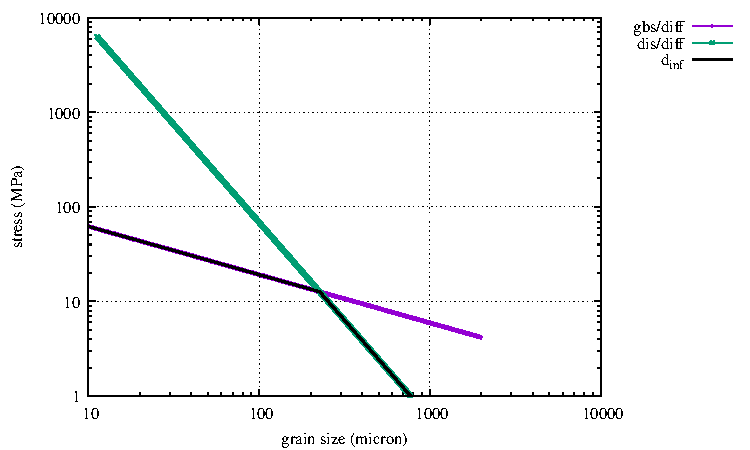
\includegraphics[width=7cm]{images/dinf/dinf.pdf}
\end{center}


\end{itemize}

The term $\dot{d}$ can be discretised by means of a simple 1st order scheme so that 
\[
\frac{d^k -d^{k-1}}{\delta t}=
-\frac{\dot\varepsilon}{\dot\varepsilon_T} (d^{k-1}-d_\infty)
\]
where $k$ is the time step index. In the end, we can update the grain size 
for each grain as follows:
\[
d^k = 
-\frac{\dot\varepsilon}{\dot\varepsilon_T} (d^{k-1}-d_\infty) \delta t + d^{k-1}
\]
This is carried out in the \lstinline{gs_evolution} function.

%%%%%%%%%%%%%%%%%%%%%%%%%
\section{shear heating}

For incompressible materials, and neglecting diffusion and advection processes, the energy equation is then
\[
\rho C_p \frac{\partial T}{\partial t} = 2 \eta \dot{\bm \varepsilon}:\dot{\bm \varepsilon}
\]
or, 
\[
\frac{\partial T}{\partial t} = \frac{2 \eta}{\rho C_p} (\dot{\varepsilon}_{xx}^2 + \dot{\varepsilon}_{yy}^2 + 2\dot{\varepsilon}_{xy}^2 ) 
\]
This means that we can write a simple post-processor that computes for each marker the maximum temperature
generated by shear heating. Of course in the absence of diffusion this remains an upper bound only meant 
to provide us with a rough estimate.


\newpage
\printbibliography
\end{document}
